\section{Approach}
\label{sec:algo}
%In this section we first give an overview of a probabilistic taxonomy
%that provides the vocabulary of concepts to abstract the verb arguments.
%as well as probabilistic scores for computing various rankings.
We first present two different confidence functions, and then
a branch-and-bound algorithm to approximately solve the
action conceptualization problem in large scale.
%Finally, we provide a method to rank the
%output action concepts from solution of action conceptualization.
In the rest of this section, the term ``argument'' refers to either
the object or the subject of a verb.

\subsection{Confidence Functions}
To define the confidence function $g_v$ for a verb $v$,
we suppose that the arguments that are relevant and correct to the verb
are more ``informative'' than those that are not.
For example, as direct objects, ``basketball'' is more informative to the verb
``play'' than ``weekend'',
because ``basketball'' appears frequently in the context of the ``play'', but
not as frequently in the context of many other verbs; while ``weekend''
appears frequently not only next to ``play'' but also to many other
verbs, such as ``go'', ``spend''.
%but does not appear in the context of many other verbs.
%However, ``weekend'' can appear in the context of many
%verbs according to the wrong parsing (e.g., recognized as the object of
%``play'', ``go'', ``buy'', etc.). According to the above observations,
Inspired by such observation, we propose two confidence functions.

\textbf{Mutual Information} is a measure in information theory which can
capture the strength of mutual connection between two terms.
In this paper, we can use the binary version of
the mutual information $MI_v$ in place of $g_v$:
\begin{equation}
MI_v(e)=
\begin{cases}
1 & \mbox{if}~\ p(v,e)\log \frac{p(v,e)}{p(v)p(e)}> 0,\\
-1 & \rm{otherwise}
\end{cases}
\end{equation}
The probability $p(v,e)$ is the co-occurrence probability
of $v$ and $e$ in the corpus, $p(v)$ and $p(e)$ are
the occurrence probabilities of $v$ and $e$ in corpus.

\textbf{TF-IDF} is a confidence scoring function in information
retrieval to identify the importance of a term to a document.
We use TF-IDF to measure the confidence of $e$ as the importance
of $e$ to the verb $v$. Specifically, $g_v$ can be defined as:
\begin{equation}
TFIDF_v(e) = freq(v,e)\cdot \log\frac{\rm{\#\ of\ verbs}}{|\{v|e\in A_v\}|},
\end{equation}
where function $freq$ is the number of times $v$ and $e$ co-occur
in the corpus.

%\subsection{A Probabilistic IsA Taxonomy}
%In this work, we use a probabilistic isA taxonomy called Probase
%\cite{WuLWZ12} which is public for download.
%Probase is a large collection of concept-subconcept (e.g., company vs.
%tech company) or concept-entity (e.g., company vs. microsoft) pairs
%which were extracted automatically by the Hearst pattern \cite{Hearst92}
%from a large web corpus.
%Probase also associates with each pair: a {\em frequency} in which
%the pair appears in the corpus, a {\em typicality score} which is
%essentially the conditional probabilities $p(e | c)$ and $p(c | e)$,
%where $c$ and $e$ represent ``concept'' and ``entity'', respectively.
%This taxonomy provide a large universe of concepts which
%our algorithms will search against to find the minimum set of concepts
%to cover a verb's arguments. Furthermore, the typicality score allows
%the algorithms to determine the importance of a concept given an entity
%and vice versa.

%\subsection{A Greedy Solution}
%\label{sec:greedy}
%The greedy solution comes up with greedily select the concept with
%smallest score according to \eqnref{eq:objfunc}.
%%Our first attempt at the NP-hard action conceptualization problem
%%is a greedy algorithm.
%%It follows a heuristic to select one concept from a candidate set
%%at a time until the final concept set is formed that covers all
%%the input arguments.
%%The candidate set can be all concepts in Probase.
%%The algorithm first creates two argument sets
%%$L$ and $D$. $L$ contains all arguments waiting to be covered
%%and $D$ contains all the arguments already covered. Initially,
%%$L$ is the set of all input arguments, and $D$ is empty.
%%In each iteration, the algorithm selects and remove a concept from
%%the candidate set which covers most arguments
%%in $L$ and least objects in $D$ while satisfy the overlap constraint
%%(see \eqnref{eq:overlap}) at the same time.
%%
%%For practical purpose, we use a reduce candidate set which contains only
%%those concepts that are in Probase and are also in the input
%%argument set. We do this primarily to speed up the computation and
%%our experiment shows that it doesn't affect the overall quality of
%%the solution.
%%%If an object is a concept in Probase, like ``clothing'', ``jewelry'' for
%%%verb ``wear'', and ``food'', ``meal'' for verb ``eat'', we put them
%%%in the candidate concept set for ``wear'' and ``eat''.
%%% \KZ{But where do we select this concept from? What is the candidate set?}
%%The newly selected concept is added to the {\em selected concept list}
%%(SCL) and all the arguments covered by the selected concept are moved
%%from $L$ to $D$ before the next iteration starts.
%%The iteration ends when $L$ is empty.
%%If $L$ is not empty, and there's no concepts in the candidate set
%%that doesn't violate the overlap constraint, then there's no
%%solution to the problem. The details of this greedy solution is shown
%%in Algorithm \ref{vega}.
%%no more
%%concepts can be added to $SCL$ because all the remaining concepts
%%violate the overlap constraint with concepts in $SCL$.
%%$L$ may be non-empty when the iteration ends.
%%As a special case, objects still in $L$ are selected as
%%concepts without considering the overlap constraint.
%
%\begin{algorithm}[th]
%\caption{Greedy Solution}
%\label{vega}
%\begin{algorithmic}[1]
%%\Function{CalcCover}{concept,E}
%%\State $coverage \leftarrow 0$
%%\For {$e \in E$}
%%\If {$e\ isA\ concept$}
%%\State $coverage \leftarrow coverage+1$
%%\EndIf
%%\EndFor
%%\State \textbf{return} $coverage$
%%\EndFunction
%%\Statex
%%\Function{PickConcept}{leftE,doneE,candidateC}
%%\State $pickC \leftarrow NULL$, $masCover \leftarrow 0$
%%\For {$c \in candidateC$}
%%\State $leftCover \leftarrow calcCover(c,leftE)$
%%\State $doneCover \leftarrow calcCover(c,doneE)$
%%\State $cover \leftarrow leftCover-doneCover$
%%\If {$cover>maxCover$}
%%\State $maxCover \leftarrow cover$
%%\State $pickC \leftarrow c$
%%\EndIf
%%\EndFor
%%\State \textbf{return} $pickC$
%%\EndFunction
%%\Statex
%%\Function{Process}{corpusE,candidateC}
%%\State $L \leftarrow corpusE$, $D \leftarrow \emptyset$
%%\State $SCL \leftarrow \emptyset$
%%\Repeat
%%\State select $c$ from $candidateC$ covering most arguments in $L$ and least in $D$ which satisfies constraint
%%\For {$e$ isA $c$}
%%\State delete $e$ from $L$
%%\State add $e$ to $D$
%%\EndFor
%%\State add $c$ to $SCL$
%%\State delete $c$ from $candidateC$
%%\Until{$L = \emptyset$}
%%\State \textbf{return} $SCL$
%%\EndFunction
%%\end{algorithmic}
%%\end{algorithm}
%\Function{Process}{corpusE,candidateC,K}
%\State $SCL \leftarrow \emptyset$
%\Repeat
%\State $S\leftarrow \emptyset$
%\For {$c\not\in SCL$}
%\State $Score\leftarrow 0$
%\For {$c'\in SCL$}
%\State $Score\leftarrow Score + Overlap(c,c')$
%\EndFor
%\State $Score\leftarrow (1-w)*Score - w*Coverage(c)$
%\State Insert $<c,Score>$ to $S$
%\EndFor
%\State Insert $c_{max}$ with smallest score to $SCL$
%\Until{$SCL.size = K$}
%\State \textbf{return} $SCL$
%\EndFunction
%\end{algorithmic}
%\end{algorithm}

%When we collect new objects, we need to update our action knowledge. Given
%a set of new collected objects, we first conduct our \emph{Action Extraction}
%on these objects to get a list of proper concepts; then we merge these concepts
%with concepts in our previous action knowledge.

%\subsection{Clustering}


%\subsection{Local Search by Simulated Annealing}
\label{sec:algo_ls}

We first build an IsA graph from the entities/concepts in each specific argument of a verb \footnote{This graph is actually a subgraph of the
Probase graph.}. As shown in \figref{fig:subgraph}, the graph is
a directed graph between the object instances of ``wear'' where each
arrow denotes an isA relation.
\begin{figure}[th]
\centering

\epsfig{file=subgraph.eps,width=0.5\columnwidth}
\caption{An IsA sub-graph for Objects of ``Wear''}
\label{fig:subgraph}
\end{figure}

Then, we propose a representative score to present how good a concept
is, by using Coverage and Inverse Typicality scores.
And below is the definition of  Coverage and Inverse Typicality:

\textbf{Coverage} - How much entities of the concept are covered by the local subgraph:
\begin{equation}
Cov(c) = \left\{ \begin{array}{ll}
1 & \textrm{, if $c \in L$}\\
\sum\limits_{e\in L}{P(e|c)=\sum\limits_{e\in L}{\frac{F(e,c)}{F(c)}}}& \textrm{, otherwise}
\end{array} \right.
\end{equation}
where $c$ is a concept, $L$ is the set of entities that appear in the local configuration, and $F(x)$ is the frequency of $x$ in Probase.

\textbf{Inverse Typicality} - How likely the concept to be the typical concept of the entities:
\begin{eqnarray}
IT(c)
&=& \frac{\sum_{e\in L}{P(e|L)P(c|e)+P(c|L)P(e|c)}}{\sum_{e\in L}{P(e|L)+\sum_{e_i}{P(c_i|L)P(e|c_i)}}} \nonumber\\
&=& \frac{\sum_{e\in L}{(F_l(e)\times \frac{F(e,c)}{F(e)}+F_l(c)\times \frac{F(e,c)}{F(c)})}}{\sum_{e\in L}{(F_l(e)+\sum_{c_i\in L}{F_l(c_i)\times \frac{F(e,c_i)}{F(c_i)}})}}
\end{eqnarray}
Where $F_l(x)$ is the local frequency of $x$. $L$ means the list of the objects of the given verb.

So the representative score of a concept $c$ is computed as follows:
\begin{equation}
RS(c) = Cov(c) \times IT(c)\times F_l(c)
\end{equation}

Because the action conceptualization problem is hard, we propose a
local search based approach here.
This approach has two steps: Initialization by a greedy method and
local search by Simulated Annealing.
Next we discuss each step in detail.


\subsubsection{Initialization}
In order to get a good initial solution, we do the initialization process by a greedy method. Our algorithm first ranks the candidate concepts by representative score from largest to smallest. As in \secref{sec:greedy},
our candidates are all those concepts in Probase which are in the
input arguments.   
We then select the concepts one by one according to the ranking above
as long as they satisfy the overlap constraint among the selected 
concepts, until all the arguments in the input are covered. 
Details is shown in Algorithm \ref{initialization}.
%\begin{algorithm}[th]
%\caption{Initialization by greedy method}
%\label{initialization}
%\begin{algorithmic}[1]
%\Function{CheckCover}{corpusE,conceptList}
%\State $flag \leftarrow true$
%\For{$e \in corpusE$}
%\State $flag' \leftarrow false$
%\For{$c \in conceptList$}
%\If{$e\ isA\ c$}
%\State $flag' \leftarrow true$, \textbf{break}
%\EndIf
%\EndFor
%\If{$flag'=false$}
%\State $flag \leftarrow false$, \textbf{break}
%\EndIf
%\EndFor
%\State \textbf{return} $flag$
%\EndFunction
%\Statex
%\Function{CheckOverlap}{$c_1$,$c_2$,overlapRate}
%\State $l_1 \leftarrow size(c_1)$, $l_2 \leftarrow size(c_2)$
%\State $l_{min} \leftarrow min(l_1,l_2)$, $sum \leftarrow 0$
%\If{$l_1 \leq l_2$}
%\For{$e \in entities\ of\ l_1$}
%\If{$e\ isA\ l_2$}
%\State $sum \leftarrow sum+1$
%\EndIf
%\EndFor
%\Else
%\For{$e \in entities\ of\ l_2$}
%\If{$e\ isA\ l_1$}
%\State $sum \leftarrow sum+1$
%\EndIf
%\EndFor
%\EndIf
%\If{$sum/l_{min} \leq overlapRate$}
%\State \textbf{return} $true$
%\Else
%\State \textbf{return} $false$
%\EndIf
%\EndFunction
%\Statex
%\Function{Initialization}{corpusE,candidateC,overlapRate}
%\State $initialC \leftarrow \emptyset$
%\State $rank\ candidateC\ by\ representative\ score$
%\For{$c \in candidateC$}
%\State $coverAll \leftarrow CheckCover(corpusE,initialC)$
%\If{$coverAll=true$}
%\State \textbf{break}
%\EndIf
%\State $flag \leftarrow true$
%\For{$c' \in initialC$}
%\State $overlap \leftarrow CheckOverlap(c,c',overlapRate)$
%\If{$overlap=false$}
%\State $flag \leftarrow false$, \textbf{break}
%\EndIf
%\EndFor
%\If{$flag=true$}
%\State $add\ c\ to\ initialC$
%\EndIf
%\EndFor
%\State \textbf{return} $initialC$
%\EndFunction
%\end{algorithmic}
%\end{algorithm}
%\begin{algorithm}[th]
%\caption{Initialization by greedy method}
%\label{initialization}
%\begin{algorithmic}[1]
%\Function{CheckCover}{corpusE,conceptList}
%\State $flag \leftarrow true$
%\For{$e \in corpusE$}
%\State $flag' \leftarrow false$
%\For{$c \in conceptList$}
%\If{$e\ isA\ c$}
%\State $flag' \leftarrow true$, \textbf{break}
%\EndIf
%\EndFor
%\If{$flag'=false$}
%\State $flag \leftarrow false$, \textbf{break}
%\EndIf
%\EndFor
%\State \textbf{return} $flag$
%\EndFunction
%\Statex
%\Function{CheckOverlap}{$c_1$,$c_2$,overlapRate}
%\State $l_1 \leftarrow size(c_1)$, $l_2 \leftarrow size(c_2)$
%\State $l_{min} \leftarrow min(l_1,l_2)$, $sum \leftarrow 0$
%\If{$l_1 \leq l_2$}
%\For{$e \in entities\ of\ l_1$}
%\If{$e\ isA\ l_2$}
%\State $sum \leftarrow sum+1$
%\EndIf
%\EndFor
%\Else
%\For{$e \in entities\ of\ l_2$}
%\If{$e\ isA\ l_1$}
%\State $sum \leftarrow sum+1$
%\EndIf
%\EndFor
%\EndIf
%\If{$sum/l_{min} \leq overlapRate$}
%\State \textbf{return} $true$
%\Else
%\State \textbf{return} $false$
%\EndIf
%\EndFunction
%\Statex
%\Function{Initialization}{corpusE,candidateC,overlapRate}
%\State $initialC \leftarrow \emptyset$
%\State $rank\ candidateC\ by\ representative\ score$
%\For{$c \in candidateC$}
%\State $coverAll \leftarrow CheckCover(corpusE,initialC)$
%\If{$coverAll=true$}
%\State \textbf{break}
%\EndIf
%\State $flag \leftarrow true$
%\For{$c' \in initialC$}
%\State $overlap \leftarrow CheckOverlap(c,c',overlapRate)$
%\If{$overlap=false$}
%\State $flag \leftarrow false$, \textbf{break}
%\EndIf
%\EndFor
%\If{$flag=true$}
%\State $add\ c\ to\ initialC$
%\EndIf
%\EndFor
%\State \textbf{return} $initialC$
%\EndFunction
%\end{algorithmic}
%\end{algorithm}

\begin{algorithm}[th]
\caption{Greedy Initialization}
\label{initialization}
\begin{algorithmic}[1]
\Function{Initialization}{corpusE, candidateC, maxOverlap}
\State $initialC \leftarrow \emptyset$
\State rank $candidateC$ by representative score
\For{$c \in candidateC$}
\If{$candidateC$ can cover all entities in $corpusE$}
\State \textbf{break}
\EndIf
\If{$c \cap c_i \le maxOverlap$ for all $c_i$ in $initialC$}
\State add $c$ to $initialC$
\EndIf
\EndFor
\State \textbf{return} $initialC$
\EndFunction
\end{algorithmic}
\end{algorithm}

%As a special case, if some entities have no concept to cover, they can be selected as concepts without any overlap constraints.

\subsubsection{Local Search}

In local search process, we first quantize the concept as follow:
$$
c_i =
\left[
\begin{array}{cccc}
p_{i1} & p_{i2} & \ldots & p_{in}
\end{array}
\right]
$$
where
$
p_{ij} = \left\{ \begin{array}{ll}
1 & \textrm{if $e_j$ is an entity of $c_i$}\\
0 & \textrm{if $e_j$ is not an entity of $c_i$}
\end{array} \right.
$
and $n$ is the number of entities of a verb.
Then we represent the concept space as follows:
$$
\left[
\begin{array}{c}
c_1\\
c_2\\
\vdots\\
c_m
\end{array}
\right]
=
\left[
\begin{array}{cccc}
p_{11} & p_{12} & \dots & p_{1n}\\
p_{21} & p_{22} & \dots & p_{2n}\\
\vdots & \vdots & \ddots & \vdots\\
p_{m1} & p_{m2} & \dots & p_{mn}
\end{array}
\right]
$$
where $m$ is the number of concepts in the concept space of a verb. 
We call the LHS of the equation \emph{concept space} and the RHS
\emph{concept-entity matrix}.
Finally, the result concepts set is represented as \emph{concept vector} ($cv$) :
$$
cv
=
\left[
\begin{array}{cccc}
p_{1} & p_{2} & \ldots & p_{m}
\end{array}
\right]
$$
where
$
p_{i} = \left\{ \begin{array}{ll}
1 & \textrm{if $c_i$ is a concept of the verb's object}\\
0 & \textrm{if $c_i$ is not a concept of the verb's object}
\end{array} \right.
$.
%In local search process, we represent the result concepts set as concept vector ($cv$) :
%$$
%cv
%=
%\left[
%\begin{array}{cccc}
%p_{1} & p_{2} & \ldots & p_{m}
%\end{array}
%\right]
%$$
%where
%$
%p_{i} = \left\{ \begin{array}{ll}
%1 & \textrm{, if $c_i$ is a concept of the verb's object}\\
%0 & \textrm{, if $c_i$ is not a concept of the verb's object}
%\end{array} \right.
%$.

To deal with the problem, we design a Simulated Annealing (SA) 
algorithm, aimed at finding high-quality solutions. 
Simulated annealing is a popular local search meta-heuristic used to address discrete and, to a lesser extent, continuous optimization problems.
The key feature of simulated annealing is that it provides a means to escape local optima by allowing hill-climbing moves (i.e., moves which worsen the objective function value) in hopes of finding a global
optimum\cite{henderson2003theory}.
The algorithm has a local search process, it applies a neighborhood
structure to iteratively generate and evaluate a sequence of solutions.
Replacing the current solution with one in the neighborhood is
called a ``move.'' The neighborhood solutions must  
satisfy overlap and coverage constraints.
Detailed algorithm is shown in Algorithm \ref{local_search}.

\begin{algorithm}[th]
\caption{Local Search by Simulated Annealing}
\label{local_search}
\begin{algorithmic}[1]
%\Function{ConceptNum}{cvParameter}
%\State $sum \leftarrow 0$
%\For{$num \in cvParameter$}
%\State $sum \leftarrow sum+num$
%\EndFor
%\State \textbf{return} $sum$
%\EndFunction
%\Statex
\Function{LocalSearch}{corpusE,initialC,overlapRate}
\State get $cvCurrent$ from $initialC$
\State $kCurrent \leftarrow sum(cvCurrent)$
\State $cvBest \leftarrow cvCurrent$, $kBest  \leftarrow kCurrent$
\State $cvNew \leftarrow \emptyset$, $kNew \leftarrow Integer.MAX$
\State $stop \leftarrow 1$, $T \leftarrow T_0$
\While{$T \geq T_{min}$}
\If{$stop \geq stop_{max}$}
\State \textbf{break}
\EndIf
\State $bestChange \leftarrow 0$, $i \leftarrow 0$
\While{$i \leq i_{max}$}
\Repeat
\State $cvNew \leftarrow cvCurrent$
\State $index \leftarrow random(lenth(cvCurrent))$
\If{$cvNew[index]=0$}
\State $cvNew[index] \leftarrow 1$
\Else
\State $cvNew[index] \leftarrow 0$
\EndIf
\Until{$cvNew$ satisfies coverage and overlap constraints}
\State $kNew \leftarrow sum(cvNew)$
\If{$kNew \leq kCurrent$}
\State $kCurrent \leftarrow kNew$
\State $cvCurrent \leftarrow cvNew$
\If{$kNew \leq kBest$}
\State $kBest \leftarrow kNew$, $cvBest \leftarrow cvNew$
\State $bestChange \leftarrow bestChange+1$
\EndIf
\Else
\State $temp \leftarrow P(kNew,kCurrent,T)$
\If{$random()\leq temp$}
\State $kCurrent \leftarrow kNew$
\State $cvCurrent \leftarrow cvNew$
\EndIf
\EndIf
\State $i \leftarrow i+1$
\EndWhile
\State $T \leftarrow T*r$
\If{$bestChange=0$}
\State $stop \leftarrow stop+1$
\Else
\State $stop \leftarrow 1$
\EndIf
\EndWhile
\State \textbf{return} $cvBest$
\EndFunction
\end{algorithmic}
\end{algorithm}

In the process, the call $random()$ returns a random float value
in the range of $[0,1]$, and the call $random(num)$ returns a
random integer value in the range of $[0,num-1]$.
%The call $CheckCoverage(corpusE,cvNew)$ and $CheckOverlap(cvNew,overlapRate)$ checks if the new concept vector satisfies the coverage and overlap constraints.
The call $P(kNew,kCurrent,T)$ returns the acceptance probabilities
(the probability of making the transition from the current
solution to the new solution).
And the acceptance probabilities function is defined as:
\[
e^{-\alpha \times (kNew-kCurrent)/T}
\]




\subsection{Approximation of Action Conceptualization}
Solving AC is much more time consuming than finding $k$-cliques in the
concept graph $L$ because in AC, the choice of the $n$-th node in an $n$-clique
depends on the configurations of all $(n-1)$-cliques.
%rather than some summary information.
The difficulty lies in the submodular function which acts
as the objective function.
We thus approximate the problem to a maximum weighted $k$-clique finding
problem by changing the objective function
to a summation. Specifically, we change $f$ in Definition \ref{def:acw} to
\begin{equation}
\tilde{f}(C_k)=\sum_{c\in C_k}{\sum_{e\in E_c\cap A_v}{g_v(e)}}.
\label{eq:approxf}
\end{equation}

This new objective function tends to over-estimate due to the
possible overlaps between the $k$ concepts.
However, since the overlaps are bounded by $\tau$,
we can obtain a bound for the over-estimation.

%\begin{lemma}
%The score of approximated action conceptualization problem is no
%larger than $k$ times of the original action conceptualization problem.
%\end{lemma}
%\begin{proof}
%Compared to the original scoring function $f$, we repeatedly compute
%the score of an entity $g_v(e)$ for $|\{c|c\in C_k, e\in E_c\}|$ times
%in the new function $f'$.
%i.e., the number of selected concepts that cover the entity $e$ in $A_v$.
%Then we have the following relation between the two problems:
%$$
%f'(C_k)=f(C_k)+\sum_{e\in \cup_{c\in C_k}{E_c}\cap A_v}{(|\{c|c\in C_k, e\in E_c\}|-1)g_v(e)}
%$$
%In the worst case, each entity is covered by all of the $k$ selected
%concepts, i.e., $|\{c|c\in C_k, e\in E_c\}|=k$. Then we obtain a simpler
%bound: $f'(C_k)<=f(C_k)+(k-1)f(C_k)=kf(C_k)$.
%\end{proof}

\begin{lemma}
The approximation ratio of $\tilde{f}(C_k)$ over $f(C_k)$ is
\[\max \left\{
	\frac{2k + (k^2 + k) \tau}{2k - (k^2 + k) \tau},
	\frac{(k-1)\tau + 2}{(k-1)\tau}\right\}.\]
\end{lemma}
\begin{proof}
First, let us assume that for any $c \in C_k$, $E_c \cap A_v$ is a uniform
sample of $E_c$.\footnote{This is a reasonable assumption because the arguments
are extracted from large text corpus which is independent from the taxonomy.}
Therefore, the maximum overlap ratio $\tau$ applies
to $E_c \cap A_v$, which we call $\tilde{E_c}$ for brevity.

Next we estimate the number of times function $g_v(e)$
is calculated in $\tilde{f}(C_k)$. For ease of presentation,
we consider the average case where for all $c \in C_k$,
$\tilde{E_c}$ is of the same size, say $s$. Since then maximum overlap
between any two sets $\tilde{E_{c1}}$ and $\tilde{E_{c2}}$ is $s\tau$,
$g_v(e)$ is thus computed at most $ks + {k\choose 2}s\tau$ times.
Whereas in the original $f(C_k)$,
$\bigcup_{c \in C_k} E_c \cap A_v$
is as small as $\min\{ks - {k\choose 2}s\tau, {k\choose2}s\tau\}$.
Therefore the approximation ratio is
\[\frac{\tilde{f}(C_k)}{f(C_k)} = \max \left\{
	\frac{2k + (k^2 + k) \tau}{2k - (k^2 + k) \tau},
	\frac{(k-1)\tau + 2}{(k-1)\tau}\right\}
\]
\end{proof}

\begin{algorithm}[th]
\caption{Branch-and-Bound on Action Conceptualization}
\label{al:backtrack}
\begin{algorithmic}[1]
\Function{AC}{$A_v, C, L, k$}
\State $\{c_0,...,c_{|C|-1}\}\leftarrow$ Sort concepts $c\in C$ in\ the\ descending\ order\ of $Score_v(c)$.
\State $\pi_{max} \leftarrow 0,\pi_{c} \leftarrow 0,ck \leftarrow 0$
\State $d_{max}\leftarrow\{0,...,0\},d\leftarrow\{0,...,0\}$
\State BB($0$)
\If{$ck = k$}
\State \textbf{return} $d_{max}$
\Else
\State \textbf{No solution}
\EndIf
\EndFunction
\Statex
\Function{BB}{$i$}
\If{$i\geq |C|$}
\State \textbf{return}
\EndIf
\If{$ck = k$}
\If{$\pi_{c}>\pi_{max}$}
\State $\pi_{max} \leftarrow \pi_{c}, d_{max} \leftarrow d$
\EndIf
\State \textbf{return}
\EndIf
\If{ISCLIQUE($L,i$) $= TRUE$ and BOUND($i$)$>\pi_{max}$}
\State $ck \leftarrow ck+1, \pi_{c} \leftarrow \pi_{c}+Score_v(c_i), d_i \leftarrow 1$
\State BB($i+1$)
\State $ck \leftarrow ck-1, \pi_{c} \leftarrow \pi_{c}-Score_v(c_i), d_i \leftarrow 0$
\EndIf
\If{BOUND($i+1$) $> \pi_{max}$}
\State $d_i \leftarrow 0$
\State BB($i+1$)
\EndIf
\State \textbf{return}
\EndFunction
\Statex
\Function{ISCLIQUE}{$L, i$}
\For{$j$ from $0$ to $i-1$}
\If{$d_j = 1$}
\If{$(c_i, c_j)\not\in L$ and $(c_j, c_i)\not\in L$}
\State \textbf{return} $FALSE$
\EndIf
\EndIf
\EndFor
\State \textbf{return} $TRUE$
\EndFunction
\Statex
\Function{BOUND}{$i$}
\State $b \leftarrow \pi_{c}$
\For{$j$ from $i$ to $\min\{i+k-ck-1, |C|-1\}$}
\State $b \leftarrow b+Score_v(c_{j})$
\EndFor
\State \textbf{return} $b$
\EndFunction
\end{algorithmic}
\end{algorithm}

\subsection{A Branch-and-Bound Algorithm}
We propose a branch-and-bound algorithm to solve the approximated
action conceptualization problem.
The complete algorithm is shown in Algorithm \ref{al:backtrack}.
We model a solution as a binary vector of size $|C|$ in which exactly
$k$ elements of the vector is set to 1 while others set to 0.
%Backtracking is a general algorithm
%that incrementally builds candidate solutions, and
%abandons each partial candidate $c$ (``backtracks'') when it determines
%that $c$ cannot be completed to a valid solution.
The search space is represented by a decision tree
where the nodes at each level represent the decision to include a concept in
the solution or not. An example of the decision tree
is shown in \figref{fig:search_tree}. The symbol $d_i$
means the binary decision on concept $c_i$. A path in
the tree is a potential solution.

\begin{figure}[th]
\centering
\epsfig{file=figure/search_tree.eps,width=0.6\columnwidth}
\caption{A snapshot of the search tree for the
example graph in \figref{fig:graph_model} with constraint $k=3$}
\label{fig:search_tree}
\end{figure}

Suppose the partial solution of the first $i$ levels in the tree
are $(d_0, d_1, ..., d_{i-1})$ and
the current best solution has a score (computed by \eqnref{eq:approxf}).
We use $d_{max}$ and $\pi_{max}$ to store the
best solution and its score found thus far; and use $d$ and $\pi_{c}$ to
represent the current partial solution and its partial score.
Variable $ck$ stands for the number of concepts that have been set to
1 in the current decision path, i.e.,
\[ck=\sum_{n=0}^{i-1}d_n.\]

The main function BB($i$) searches through the tree in a depth-first manner.
It returns when it reaches the leaf node (Line 11-12) or when it has found a
solution (Line 13-16). If the solution is better than the current best,
the current best solution is updated. The function traverses one
more level to include concept $c_i$ (Line 17-19) if it forms
a clique with the currently chosen concepts (ISCLIQUE function)
and if the maximum possible score with $c_i$ is better than
the current best score (BOUND function). It backtracks to exclude $c_i$
when the left branch is searched (Line 20-23).

A crucial optimization in this algorithm is that we first sort
all concepts in $C$ decreasingly by their weighted score (Line 2),
\[Score_v(c) = \sum_{e\in E_c \cap A_v} g_v(e),\]
which is a component in \eqnref{eq:approxf}. This allows us to quickly
compute the bound (Line 33-34) in linear time (against $k$), i.e., simply
the total score of the next $k-ck$ concepts down the decision
tree hierarchy, rather than sorting all the remaining concepts,
which is a much larger set.

For pure illustration purpose, we explore
the search space and the pruning ratio (number of nodes traversed with
bounds versus without bounds) by simulating the execution
of the algorithm on proportionally smaller inputs, i.e., smaller
number of concepts, smaller concepts and fewer edges in the graph.
The pruning ratio versus the average concept size and
the input $k$ is shown in \figref{fig:complexity}.
In practice, pruning search space by this bounding mechanism turns
out to be very effective.The execution times of the algorithm are
very reasonable under various experimental settings,
shown in \secref{sec:efficiency}.

\vspace*{-10mm}
\begin{figure}[th]
\centering
\epsfig{file=figure/complexity_data.eps,width=0.7\columnwidth}
\caption{Pruning ratio over average concept size and $k$}
\label{fig:complexity}
\end{figure}

%The decision tree is pruned under two conditions:
%1) if the subgraph formed by the selecting concept $i$ is not a
%clique or the size is larger than $k$,
%then do not need to check the $i+1$ concept (Line 10-17);
%2) if the maximum possible score for the decision that \emph{without} selecting concept $i$
%is smaller than $\pi_{max}$, then do not need to check the $i+1$ concept (Line 18-20).
%The computation of maximum possible score on a path with less than $k$
%concepts selected is to choose the top $k-ck$ concepts with maximum scores.
%%Otherwise, we stop traversing the subtree under the decision $d_i=1$.
%In order to efficiently find the top $k-ck$ concepts, we first
%compute all the $Score_v(c)$ for all the concepts and sort the
%concepts in the descending order of $Score_v(c)$. When we search for top $n$ concepts
%in the descendants of the $i$-th concept,
%we pick the ($i+1, i+2, ..., i+n$) concepts.

%\subsection{Weighted Sum Solution}
%\label{sec:algo_weightedsum}
%
%As our problem is a multi-objective programming problem, we can solve it by a Weighted Sum Solution. A weight $w$ which demonstrates the optimization preference to \textbf{Coverage} and \textbf{Overlap} is first given by the decision maker. So the problem can be reformulated to a single-objective problem and is formalized as follow, we call it AC-QP.
%\begin{eqnarray}
%\min_{x} && (1-w)x^TPx-wd^Tx \label{eq:objfunc}\\
%\rm{subject~to} && x_s(x_s-1)=0\\
%&&\sum_{s\in S}{x_s}=k
%\end{eqnarray}
%
%In the definition above, the equation $x_s(x_s-1)=0$ is non-convex quadratic constraint, so the problem is a case of non-convex QCQR.
%
%Then the equivalent SDP(semidefinite programming) formulation of AC-QP can be indicated as following, we call it AC-SDP.
%\begin{eqnarray}
%\min_{X,x} && Q\bullet X+c^Tx \label{qcqpsubj}\\
%\rm{subject~to} && e^Tx=k\\
%&&diag(X)=x\\
%&&X=xx^T
%\end{eqnarray}
%where $Q\bullet X=trace(QX)=\sum\limits^n_{i=1}\sum\limits^n_{j=1}{Q_{ij}X_{ij}}$ and $Q=(1-w)P, c=-wd$.
%
%Because we have nonconvex constraints in AC-SDP, so $X=xx^T$ is relaxed to $X-xx^T\succeq 0$. And then the semidefinite relaxation of AC-QP is obtained as following, we call it AC-SDR.
%\begin{eqnarray}
%\min_{X,x} && Q\bullet X+c^Tx \\
%\rm{subject~to} && e^Tx=k\\
%&&diag(X)=x\\
%&&\left[
%\begin{array}{cc}
%1 & x^T\\
%x & X
%\end{array}
%\right]\succeq 0
%\end{eqnarray}

%\subsection{Quadratic Convex Reformulation}
%Since our problem has non-convex constraints, we use a \emph{Quadratic Convex Reformulation} (QCR)
%to reformulate the problem to a convex one. This method apply a continuous relaxation to the 0-1
%constraint, i.e., we weaken the 0-1 constraint to $0\leq x_i \leq 1$. After continuous relaxation,
%we need to reformulate the original problem to make the lower bound of continuous relaxation equal
%to the lower bound of Semi-Definite Program relaxation. Suppose strong duality holds for the SDP relaxation
%and a dual optimal solution ($\lambda^*, \mu^*$) exists, if we perturb the objective function
%\ref{qcqpsubj} by:
%\begin{itemize}
%\item adding $x^Tdiag(\lambda^*)x-(\lambda^*)^Tx$ and $\mu^*(e^Tx-k)$
%\item changing the equality constraints to inequality constraints with opposite sign,
%\end{itemize}
%then the reformulated problem is convex and the lower bound of the continuous relaxation equals to
%the lower bound of SDP relaxation. The reformulated problem is shown as follows:
%\begin{eqnarray}
%\min_{x} && (1-w)x^TPx-wd^Tx \nonumber \\
%&&+x^Tdiag(\lambda^*)x-(\lambda^*)^Tx \nonumber\\
%&&+\mu^*(e^Tx-k) \\
%\rm{subject~to} && e^Tx\leq k\\
%&& e^Tx\geq k\\
%&& 0\leq x_s \leq 1, for all s\in S
%\end{eqnarray}

%\subsection{Graph Based Approach}
%\begin{eqnarray*}
%\max_{x} && \sum_{s\in S}{Coverage(s)\cdot x_s} \\
%\rm{subject~to} && x_s\cdot (x_s-1)=0\\
%&&\sum_{s\in S}{x_s}=k\\
%&& Overlap(s,t)\cdot x_t\cdot x_s\leq \tau, for\ all\ s,t\in S, s\neq t
%\end{eqnarray*}
%
%\subsubsection{Graph Representation}
%Let us consider the following graph representation of a set $S$ of concepts. Let $G_{S,\tau}=(V,E)$ be an undirected graph such that there is a vertex $v_i\in V$ for each concept $s_i\in S$ with the weight $w(v_i)=Coverage(s_i)$ and an edge $(v_i,v_j)\in E$, if and only if, $Overlap(s_i,s_j)\leq \tau$ for the corresponding concepts $s_i,s_j,s_i\neq s_j$. An example is shown in \figref{fig:graph_model}.
%\begin{figure}[th]
%\centering
%\epsfig{file=figure/graph_model.eps,width=1.0\columnwidth}
%\caption{(a) Concept set $S$ with overlap constraint $\tau$ as the radius and (b) the corresponding graph representation $G_{S,\tau}$}
%\label{fig:graph_model}
%\end{figure}
%
%Let us recall a couple of graph-related definitions. A \emph{complete subgraph} $D$ in a graph $G$ is a subgraph of $G$ such that every two vertices in $D$ are joined by an edge. And a \emph{maximum complete subgraph} is such a subgraph of $G$ with the maximum sum of vertices weight.
%
%Considering the definition of \emph{action conceptualization} problem, solving such problem is equivalent to finding a \emph{maximum complete subgraph} with $k$ vertices in the corresponding graph  $G_{S,\tau}$, we call it \emph{graph based action conceptualization} problem.




%\subsection{Ranking of Action Concepts}
\label{sec:rank}
Previous two algorithms return an approximately  minimum set of
concepts that cover all the input argument instances of a given verb
which satisfy the overlap constraint. This subsection introduce a
simple but effective way to rank these concepts. This ranking is
important for three reasons.
I think ranking has the following purposes:
\begin{enumerate}
\item There are still many concepts (in the hundreds) in the AC results,
thus there is need to present the most representative concepts for
human consumption;
\item Not all the concepts are useful in argument identification,
as we will point out later in \secref{sec:eval}, the top concepts for
an argument are often sufficient to determine whether an argument is
legal and correct.
\item There are noisy concepts which are too general and often contain
incorrect entities due to the inaccuracy of dependency parsers. A
good ranking algorithm may ``rank down'' these undesirable concepts.
\end{enumerate}

The basic idea behind our ranking algorithm is that the best concept
(the concept that has the largest representative score) has the highest
priority to pick the arguments in corpus. After one argument is
picked by a concept, it will be removed from the candidate argument set
(CAS). And the iteration ends up when CAS is empty.
In this process, every concept has an attribute named $CN$
which is the number of unique entities a concept covers.
Finally, $CN$ is used as criterion to rank the concepts.
Our algorithm is shown in Algorithm \ref{rank_concepts}.

\begin{algorithm}[th]
\caption{Rank concepts}
\label{rank_concepts}
\begin{algorithmic}[1]
\Function{RankConcepts}{corpusE,resultC}
\State rank $resultC$ by representative $score$
\For{$c \in resultC$}
\State $num \leftarrow 0$
\For{$e \in corpusE$}
\If{$e\ isA\ c$}
\State $num \leftarrow num+1$
\State remove $e$ from $corpusE$
\EndIf
\EndFor
\State $c.CN\leftarrow num$
\EndFor
\State rank $resultC$ by $CN$
\State \textbf{return} $resultC$
\EndFunction
\end{algorithmic}
\end{algorithm}


